% Understanding the DFT and its inverse acting on real polynomials
% Author: Max Sills
\documentclass[landscape]{article}
\usepackage{tikz}
\usepackage[top=1in,bottom=1in,right=1in,left=1in]{geometry}
\begin{document}
    \begin{tikzpicture}[scale=2,cap=round,>=latex]
        % draw the coordinates
        \draw[->] (-1.5cm,0cm) -- (1.5cm,0cm) node[right,fill=white] {$x$};
        \draw[->] (0cm,-1.5cm) -- (0cm,1.5cm) node[above,fill=white] {$y$};

        % draw the unit circle
        \draw[thick] (0cm,0cm) circle(1cm);

        
        %draw roots of unity
         \foreach \x/\xtext/\y in {
            % the coordinates for the first quadrant
            0/a + b + c}
                \draw (\x:1.25cm) node[fill=white] {$\left(\xtext\right)$};
        
  \end{tikzpicture}
  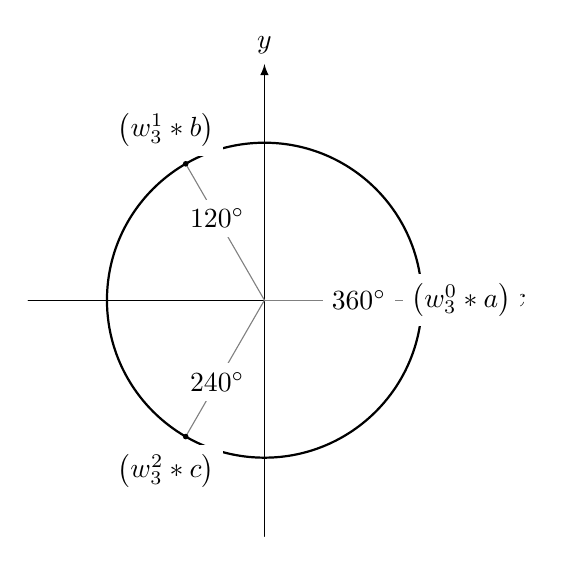
\begin{tikzpicture}[scale=2,cap=round,>=latex]
        % draw the coordinates
        \draw[->] (-1.5cm,0cm) -- (1.5cm,0cm) node[right,fill=white] {$x$};
        \draw[->] (0cm,-1.5cm) -- (0cm,1.5cm) node[above,fill=white] {$y$};

        % draw the unit circle
        \draw[thick] (0cm,0cm) circle(1cm);

        %draw radian lines
        \foreach \x in {0,120,...,360} {
                % lines from center to point
                \draw[gray] (0cm,0cm) -- (\x:1cm);
                % dots at each point
                \filldraw[black] (\x:1cm) circle(0.4pt);
                % draw each angle in degrees
                \draw (\x:0.6cm) node[fill=white] {$\x^\circ$};
        }
        
        %draw roots of unity
         \foreach \x/\xtext/\y in {
            % the coordinates for the first quadrant
            0/w^{0}_{3} * a,
            120/w^{1}_{3} * b,
            240/w^{2}_{3} * c}
                \draw (\x:1.25cm) node[fill=white] {$\left(\xtext\right)$};
        
    \end{tikzpicture}
    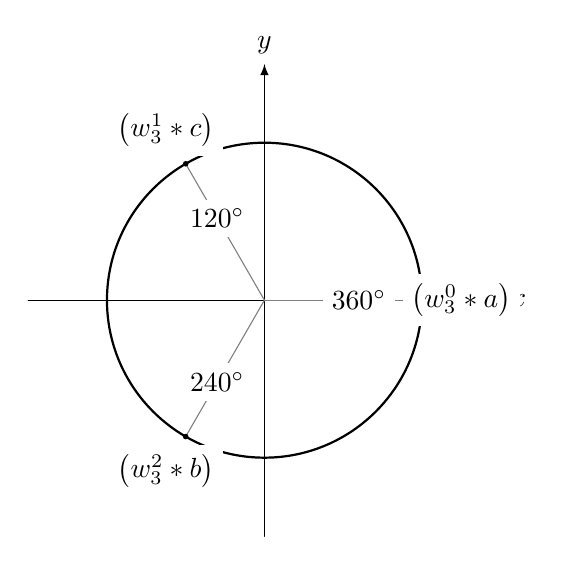
\begin{tikzpicture}[scale=2,cap=round,>=latex]
        % draw the coordinates
        \draw[->] (-1.5cm,0cm) -- (1.5cm,0cm) node[right,fill=white] {$x$};
        \draw[->] (0cm,-1.5cm) -- (0cm,1.5cm) node[above,fill=white] {$y$};

        % draw the unit circle
        \draw[thick] (0cm,0cm) circle(1cm);

        %draw radian lines
        \foreach \x in {0,120,...,360} {
                % lines from center to point
                \draw[gray] (0cm,0cm) -- (\x:1cm);
                % dots at each point
                \filldraw[black] (\x:1cm) circle(0.4pt);
                % draw each angle in degrees
                \draw (\x:0.6cm) node[fill=white] {$\x^\circ$};
        }
        
        %draw roots of unity
         \foreach \x/\xtext/\y in {
            % the coordinates for the first quadrant
            0/w^{0}_{3} * a,
            120/w^{1}_{3} * c,
            240/w^{2}_{3} * b}
                \draw (\x:1.25cm) node[fill=white] {$\left(\xtext\right)$};
    \end{tikzpicture}
    
Then the inverse can scale each clock, and we can swap arm lengths between clocks because addition is commutative.

   \begin{tikzpicture}[scale=2,cap=round,>=latex]
        % draw the coordinates
        \draw[->] (-1.5cm,0cm) -- (1.5cm,0cm) node[right,fill=white] {$x$};
        \draw[->] (0cm,-1.5cm) -- (0cm,1.5cm) node[above,fill=white] {$y$};

        % draw the unit circle
        \draw[thick] (0cm,0cm) circle(1cm);

        
        %draw roots of unity
         \foreach \x/\xtext/\y in {
            % the coordinates for the first quadrant
            0/\frac{a + a + a}{3}}
                \draw (\x:1.25cm) node[fill=white] {$\left(\xtext\right)$};
        
  \end{tikzpicture}
  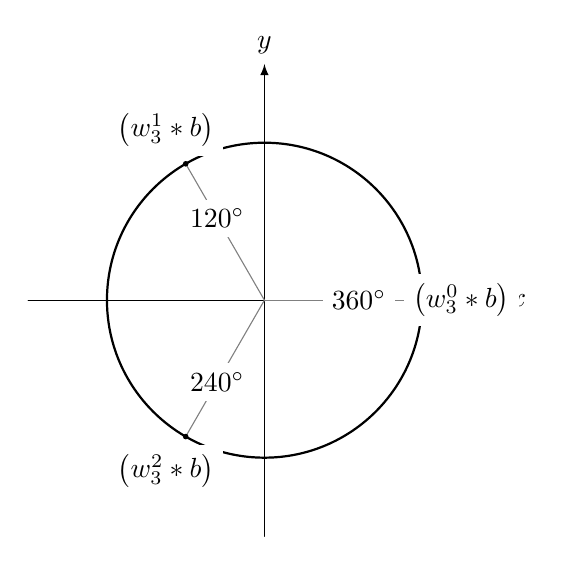
\begin{tikzpicture}[scale=2,cap=round,>=latex]
        % draw the coordinates
        \draw[->] (-1.5cm,0cm) -- (1.5cm,0cm) node[right,fill=white] {$x$};
        \draw[->] (0cm,-1.5cm) -- (0cm,1.5cm) node[above,fill=white] {$y$};

        % draw the unit circle
        \draw[thick] (0cm,0cm) circle(1cm);

        %draw radian lines
        \foreach \x in {0,120,...,360} {
                % lines from center to point
                \draw[gray] (0cm,0cm) -- (\x:1cm);
                % dots at each point
                \filldraw[black] (\x:1cm) circle(0.4pt);
                % draw each angle in degrees
                \draw (\x:0.6cm) node[fill=white] {$\x^\circ$};
        }
        
        %draw roots of unity
         \foreach \x/\xtext/\y in {
            % the coordinates for the first quadrant
            0/w^{0}_{3} * b,
            120/w^{1}_{3} * b,
            240/w^{2}_{3} * b}
                \draw (\x:1.25cm) node[fill=white] {$\left(\xtext\right)$};
        
    \end{tikzpicture}
    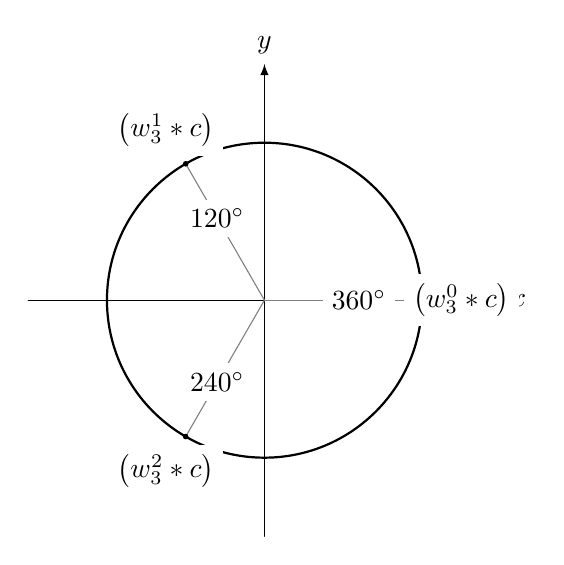
\begin{tikzpicture}[scale=2,cap=round,>=latex]
        % draw the coordinates
        \draw[->] (-1.5cm,0cm) -- (1.5cm,0cm) node[right,fill=white] {$x$};
        \draw[->] (0cm,-1.5cm) -- (0cm,1.5cm) node[above,fill=white] {$y$};

        % draw the unit circle
        \draw[thick] (0cm,0cm) circle(1cm);

        %draw radian lines
        \foreach \x in {0,120,...,360} {
                % lines from center to point
                \draw[gray] (0cm,0cm) -- (\x:1cm);
                % dots at each point
                \filldraw[black] (\x:1cm) circle(0.4pt);
                % draw each angle in degrees
                \draw (\x:0.6cm) node[fill=white] {$\x^\circ$};
        }
        
        %draw roots of unity
         \foreach \x/\xtext/\y in {
            % the coordinates for the first quadrant
            0/w^{0}_{3} * c,
            120/w^{1}_{3} * c,
            240/w^{2}_{3} * c}
                \draw (\x:1.25cm) node[fill=white] {$\left(\xtext\right)$};
    \end{tikzpicture}

The right two clocks cancel out because adding equally spaced roots of unity equals zero, and scaling zero by a real number is still zero. So the first row of the inverse DFT is $\langle$ 1, 1, 1 $\rangle$


\end{document}
